\chapter{Introdu\c{c}\~ao/motiva\c{c}\~ao}
No in�cio da transmiss�o um n� � definido como fonte. Ao entrar um n� destino (receptor da transmiss�o), o algoritmo de Floyd-Warshall � utilizado para dividir o fluxo, levando em considera��o a capacidade de cada aresta. Quando outro n� destino entrar, uma busca em largura � realizada para encontrar as partes mais pr�ximas que completam o fluxo e estas s�o transmitidas para o novo host, por um caminho determinado pelo algoritmo Floyd-Warshall. Um exemplo pode ser observado na figura 
\begin{figure}
	\centering
	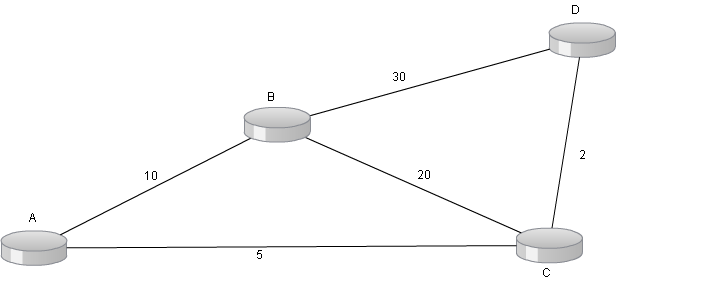
\includegraphics[scale=0.6]{Grafo_exemplo_mestrado.png}
	\caption{"Grafo exemplo de topologia"}
	\label{fig:topo_example}
\end{figure}

\section{Contextualiza��o}
\subsection{Linux}
\section{Motiva��o e Objetivos}
\subsection{Linux}
\section{Metodologia}
\subsection{Linux}
\section{Estrutura��o do texto}
\subsection{Linux}
Utilize o BibTeX para organizar as suas refer�ncias. 
